\documentclass[12pt]{article}

\usepackage[utf8x]{inputenc} % Включаем поддержку UTF8  
\usepackage[russian]{babel}  % Включаем пакет для поддержки русского языка  
\usepackage{hyperref}        % Для гиперссылок

% Математика
\usepackage{amsmath,amsfonts,amssymb,amsthm,mathtools} % AMS
\usepackage{icomma}
\usepackage{mathrsfs}

\usepackage{xcolor}

% Прога
\usepackage{etoolbox}
\usepackage{listings}

\definecolor{codegreen}{rgb}{0,0.6,0}
\definecolor{codegray}{rgb}{0.5,0.5,0.5}
\definecolor{codepurple}{rgb}{0.58,0,0.82}
\definecolor{backcolour}{rgb}{0.95,0.95,0.92}

\lstdefinestyle{mystyle}{
	backgroundcolor=\color{backcolour},   
	commentstyle=\color{codegreen},
	keywordstyle=\color{magenta},
	numberstyle=\tiny\color{codegray},
	stringstyle=\color{codepurple},
	basicstyle=\ttfamily\footnotesize,
	breakatwhitespace=false,         
	breaklines=true,                 
	captionpos=b,                    
	keepspaces=true,                 
	numbers=left,                    
	numbersep=5pt,                  
	showspaces=false,                
	showstringspaces=false,
	showtabs=false,                  
	tabsize=2
}

\lstset{style=mystyle}

% Цвета
\usepackage{xcolor}

% Картинки
\usepackage{graphicx}
\graphicspath{ {./images/} }

\usepackage{tikzsymbols}

% Работа с таблицами
\usepackage{array,tabularx,tabulary,booktabs} % Дополнительная работа с таблицами
\usepackage{longtable}  % Длинные таблицы
\usepackage{multirow} % Слияние строк в таблице

% Нумерованные списки
\usepackage[shortlabels]{enumitem} % Разные лейблы

% Текст
\usepackage[normalem]{ulem}  % для зачеркивания текста

\newtheorem{property}{Свойство}
\newtheorem{consequence}{Следствие}[property]

\usepackage{parskip}   % отступы между параграфами

\DeclarePairedDelimiter\abs{\lvert}{\rvert}%
\DeclarePairedDelimiter\norm{\lVert}{\rVert}%

% Swap the definition of \abs* and \norm*, so that \abs
% and \norm resizes the size of the brackets, and the 
% starred version does not.
\makeatletter
\let\oldabs\abs
\def\abs{\@ifstar{\oldabs}{\oldabs*}}
%
\let\oldnorm\norm
\def\norm{\@ifstar{\oldnorm}{\oldnorm*}}
\makeatother

\begin{document}
	
	\thispagestyle{empty}
	\begin{center}
		\textbf{ПРАВИТЕЛЬСТВО РОССИЙСКОЙ ФЕДЕРАЦИИ}
		
		\vspace{5ex}
		
		\textbf{Федеральное государственное автономное образовательное учреждение \\ высшего образования \\ <<Национальный исследовательский университет \\ <<Высшая школа экономики>>}
	\end{center}
	\vspace{5ex}
	
	\begin{center}
		Московский институт электроники и математики им. А.Н. Тихонова  
		
		\vspace{5ex}
		
		Департамент прикладной математики
		
		\vspace{10ex}
		\textbf{Отчёт \\ по ребусу №1 \\ по курсу <<Алгоритмизация и программирование>>}
		\vspace{7ex}
		
	\end{center}
	
	\begin{center} 
		\begin{tabular}{| p{0.3\linewidth}| p{0.3\linewidth}| p{0.3\linewidth}|}
			\hline	
			ФИО студента & Номер группы & Дата \\  \hline
			& & \\  
			Кейер Александр \newline Петрович & БПМ-231 & \today\\  
			& & \\  \hline		
		\end{tabular}
	\end{center}
	
	\begin{center}
		\vspace{3ex}
		
		\vfill
		
		\normalsize
		
		\textbf{Москва, 2024}
	\end{center}
	
	\newpage
	
	%---------------------------------------------------------------------------------
	

	\section*{Вопрос 1}
	
	main.cpp
	\begin{lstlisting}[language=C++]
		#include "foo.h"
		int main() {
			foo();
			return 0;
		}
	\end{lstlisting}
	foo.h
	\begin{lstlisting}[language=C++]
		void foo() {
			/* some code */
		}	
	\end{lstlisting}
	foo.cpp
	\begin{lstlisting}[language=C++]
		#include "foo.h"
		
		/* some code */
	\end{lstlisting}
	
	\textbf{Проблема:} в данном случае функция foo реализована в заголовочном файлу foo.h - это не очень хорошо, поскольку если этот заголовочный файл будет включаться в несколько единиц трансляции (в ребусе включается в main.cpp и в foo.cpp), то компоновщик во время линковки выбросит ошибку, ссылающуюся на ODR (One Definition Rule), которое гласит, что функция не может быть определена более одного раза (единственный источник правды).
	
	\textbf{Решение 1:} если переписать foo.h в следующий вид,
	\begin{lstlisting}[language=C++]
		inline void foo() {
			/* some code */
		}	
	\end{lstlisting}
	то описанная проблема пропадет. То есть:
	\begin{enumerate}
		\item Этап препроцессинга - все также вставим вместо \#include ''foo.h'' все содержимое файла (но уже с inline)
		\item Этап трансляции (компиляции) - не совсем понятно как, но, видимо, благодаря inline здесь на уровне бинарных файлов единиц трансляции каким-то образом происходит разрешение коллизии.
		\item Этап линковки - здесь уже не возникает ошибок, ссылающихся на ODR
	\end{enumerate}
	
	\textbf{Решение 2:} хорошей практикой является лишь описание сигнатуры функции внутри .h файлов, а реализация этой функции должна попадать уже в зону ответственности соответствующей единицы трансляции.
	
	\textbf{Интересно:} если проводить последовательно (руками) препроцессинг, трансляцию и линковку, то ошибка возникает. Если же давать компилятору g++ самостоятельно осуществить эти этапы, то ошибки не возникает, но на уровне ассемблерного кода можно обнаружить отличие в виде двух команд (см. фото ниже). Подробнее изучить, зачем это нужно, можно по \href{https://gcc.gnu.org/legacy-ml/gcc/2003-09/msg00984.html}{ссылке}.
	
	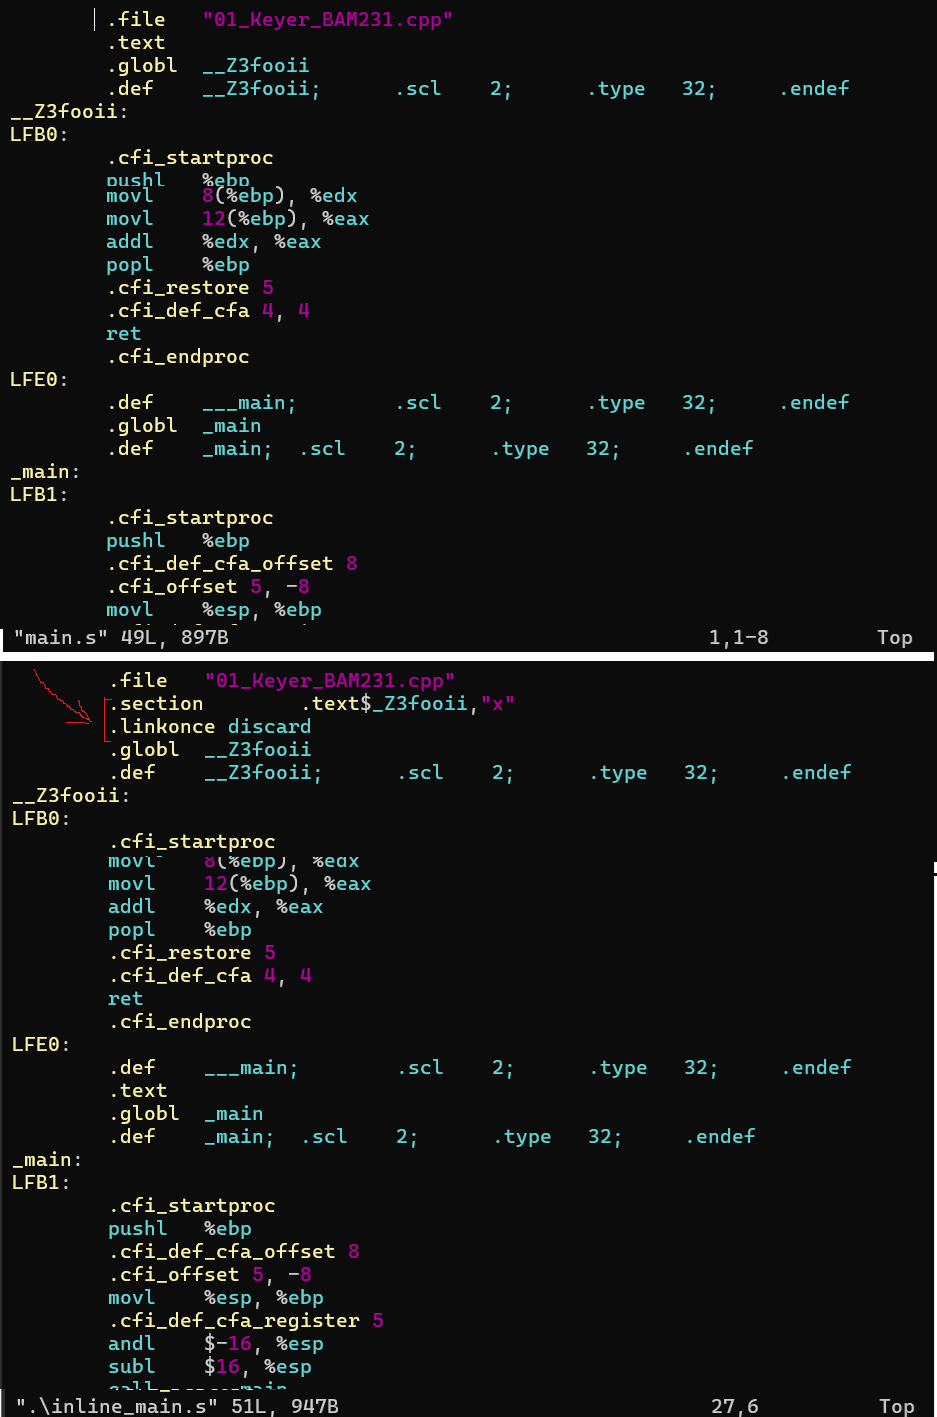
\includegraphics[width=\linewidth]{question_1.png}
	
	\section*{Вопрос 2}
	
	int a = 0, b = 1; // Объявили и инициализировали на стеке две целочисленные переменные a и b.
		
	int result = (10, (a = 3) + (b = 4)); // Используем оператор "запятая". Сначала вычисляем левый операнд - там 10, поэтому отбрасываем результат и переходим ко второму операнду. Присываиваем переменной a значение 3. Присываиваем переменной b значение 4. Вычисляем правый операнд = 3 + 4 = 7. В итоге: a = 3, b = 4, result = 7.
	
	\section*{Вопрос 3}
	
	\begin{lstlisting}[language=C++]
		int arr[3] = { 0, 2, 3 };
		
		if (arr[0] == *arr || (arr[0] = 1))
			arr[1] = 0;
	\end{lstlisting}
	
	int arr[3] = { 0, 2, 3 }; // Создали на стеке статический массив из 3 элементов.
	
	if (arr[0] == *arr || (arr[0] = 1)) // arr[0] - взяли первый элемент массива. *arr взяли значения указателя arr, который указывает на первый элемент массива. Итого левая часть условия arr[0] == *arr верна. Оператор "ИЛИ" $||$ останавливается, когда получаем первый истинный результат, поэтому до правой части (arr[0] = 1) мы не доходим.
	
	arr[1] = 0; // Условие оператора if ИСТИНА, поэтому сдвигаем указатель arr на 1 вправо и обновляем значение полученного указателя на 0. Итого получаем массив { 0, 0, 3}.
\end{document}
